% ------------ begin cheatsheet
\documentclass[a4paper]{article}
\usepackage[a4paper,margin=0.03in]{geometry}
\usepackage{multicol}

\usepackage{amsmath, amssymb}
\usepackage[inline]{enumitem}
\usepackage{graphicx}
\usepackage{xcolor}

\usepackage{ulem}
\usepackage{makecell}

% math-mode version of "c" column type
\newcolumntype{C}{>{$}c<{$}}

\newcommand{\Z}{\mathbb{Z}}

% horizontal list
\newlist{hlist}{enumerate*}{1}
\setlist[hlist]{label={}, afterlabel={}, itemjoin={{ \textbar{} }}}

% math
\newcommand{\abs}[1]{\left\lvert#1\right\rvert}
\usepackage{spalign}
\let\mat=\spalignmat
\let\amat=\spalignaugmat
\newcommand{\pp}{{\prime\prime}}
\newcommand{\sgn}[1]{\mathrm{sgn}(#1)}
\newcommand{\gen}[1]{\langle #1 \rangle}
\newcommand{\ord}[1]{\mathrm{o}(#1)}
\newcommand{\kernel}[1]{\mathrm{ker} \; #1}
\newcommand{\sub}[1]{\mathrm{\textbf{Sub}}(#1)}
\newcommand{\Aut}[1]{\mathrm{Aut}(#1)}
\newcommand{\Inn}[1]{\mathrm{Inn}(#1)}
\newcommand{\vv}{\vert\vert}

% envs
\newcommand{\oli}[1]{\begin{enumerate*}[label=(\arabic*)]#1\end{enumerate*}}
\newcommand{\yellow}[1]{\colorbox{yellow}{#1}}

\graphicspath{ {./images/} }
\pagestyle{empty}
\setlength{\columnseprule}{0.2pt}

% reduce spacing before and after headers
\newcommand{\uppercaseandunderline}[1]{\uline{\uppercase{#1}}}

\makeatletter
\renewcommand{\section}{
  \@startsection{section}{1}{0pt}{1ex}{1.2ex} {\raggedleft\normalfont\large\bfseries\uppercaseandunderline}}
\renewcommand{\subsection}{
  \@startsection{subsection}{2}{0pt}{1ex}{1.2ex} {\raggedleft\normalfont\normalsize\bfseries\fbox}}
\renewcommand{\subsubsection}{
  \@startsection{subsubsection}{3}{0pt}{1ex}{0.8ex} {\raggedleft\normalfont\footnotesize\bfseries\uline}}
\renewcommand{\paragraph}{
  \@startsection{paragraph}{4}{0pt}{1.5ex}{-0.8em}{\normalfont\bfseries}}
% ------------ end cheatsheet

\begin{document}
\footnotesize
\setlength{\abovedisplayskip}{2pt}
\setlength{\belowdisplayskip}{2pt}
\setlength{\abovedisplayshortskip}{0pt}
\setlength{\belowdisplayshortskip}{0pt}
\begin{multicols*}{3}
\section*{\centering \underline{MA2202}}
  \begin{itemize}[leftmargin=*]
    \item To prove uniqueness, suppose not unique and try to show equality.
    \item To prove equality of two sets, show that each is a subset of the other.
    \item To show that two groups are not isomorphic, prove by contradiction.
    \item Element $x$ has finite order $\implies x^a = e$ for some $a$
    \item Intersection with $A_n \implies$ only take even permutations, which have $\sgn{x} = 1$.
  \end{itemize}
  \subsubsection*{Functions} \noindent
    Let $A, B$ be sets, and let $f: A \rightarrow B$ be a function.
    \begin{itemize}[leftmargin=*]
      \item For $a \in A$, denote $f(a) = b \in B$.
      \item The set $A$ is called the domain, and the set $B$ is called the co-domain.
      \item The range/image of $f$ is
        \[ \{b \in B : b = f(a) \text{ for some } a \in A\} \]
      \item Let $B' \subseteq B$. Define
        \[ f^{-1}(B') = \{ a \in A : f(a) \in B' \} \]
      \item If $g: C \rightarrow D$ is another function, then we say $f=g \iff A=C, B=D$ and $f(a) = g(a) \; \forall a \in A$
      \item If $S \subseteq A$, then $f \vert_S$ denotes the same function except that the domain $A$ is replaced by $S$. This function $f \vert_S$ is called the restriction of $f$ to $S$.
      \item If $h: B \rightarrow C$, then the composite of $h$ and $f$ is a function $h \circ f: A \rightarrow C$ given by
        \[ (h \circ f)(a) = h(f(a)) \quad \forall a \in A \]
    \end{itemize}
    \paragraph{Notable examples}
      \begin{itemize}[leftmargin=*]
        \item The identity fn on $A$ is $f: A \rightarrow A$ defined by
          \[ f(x) = x \quad \forall x \in A \]
          We also denote the identity function on $A$ by $\mathrm{id}_A$.
        \item The inclusion fn on $Y$ for some $Y \subset X$ is the function $h: Y \rightarrow X$ defined by $h(y) = y \; \forall y \in Y$.
      \end{itemize}
    \paragraph{\yellow{Injection/Surjection/Bijection}}
      Let $f: A \rightarrow B$ be a function.
      \begin{enumerate}[leftmargin=*]
        \item $f$ is an injection if $f(a) = f(a') \implies a = a'$.
        \item $f$ is a surjection if $\forall b \in B, \exists a \in A$ s.t. $f(a) = b$.
        \item $f$ is a bijection if it is both an injection and a surjection.
        \item If $f$ is a bijection, we can define the inverse function $f^{-1}: B \rightarrow A$ in the following way: \\
          $\forall b \in B, \exists$ unique $a \in A$ such that $f(a) = b$. Then $f^{-1}(b) = a$.
        \item A fn is a bijection $\iff$ its inverse fn exists.
      \end{enumerate}
\subsection*{Integers}
  \subsubsection*{Divisibility} \noindent
    Given $a, b \in \Z$ where $a \neq 0$.
    \begin{itemize}[leftmargin=*]
      \item We say $a$ divides $b$ if $b = ma$ for some $m \in \Z$. The integer $b$ is a multiple of $a$, and we write $a|b$.
      \item An integer $n$ is called a unit if it divides 1. Hence $n = 1$ or $-1$.
      \item Transitivity holds, i.e. $a|b$ and $b|c \implies a|c$
    \end{itemize}
  \subsubsection*{Prime} \noindent
    A nonzero $p \in \Z$ is called a prime integer if:
    \begin{enumerate}[leftmargin=*]
      \item $p$ is not a unit (i.e $p \neq \pm 1$), and
      \item if $p$ divides $ab$ for some $a,b \in \Z$, then $p|a$ or $p|b$.
    \end{enumerate}
    A positive prime integer is called a prime number.
  \subsubsection*{Irreducible} \noindent
    A nonzero $p \in \Z$ is called a irreducible integer if:
    \begin{enumerate}[leftmargin=*]
      \item $p$ is not a unit (i.e $p \neq \pm 1$), and
      \item if $p$ divides $xy$ for some $x,y \in \Z$, then either $x$ or $y$ is a unit, i.e. $x$ or $y$ is $\pm 1$.
    \end{enumerate}
  \subsubsection*{Prime vs irreducible} \noindent
    Let $p$ be an integer. It is an irreducible integer $\iff$ it is a prime integer.
\subsection*{The Euclidean algorithm} \noindent
  Let $x, y \in \Z$ with $y \neq 0$. Then there exist unique integers $q$ and $r$ such that
    \[ x = qy + r \text{ and } 0 \le r < \abs{y} \]
  This is also known as the division algorithm.
  \subsubsection*{Common divisor} \noindent
    Given two integers $x$ and $y$ where $y \neq 0$.
    \begin{itemize}[leftmargin=*]
      \item A nonzero integer $m$ is called a common divisor if $m|x$ and $m|y$.
      \item $1$ is always a common divisor.
      \item If $m$ is a common divisor, $-m$ is also a common divisor.
      \item Every common divisor lies bewtween $-\abs{y}$ and $\abs{y}$.
      \item There are only finitely many common divisors.
    \end{itemize}
  \subsubsection*{Greatest common divisor} \noindent
    There is a largest number $d$ among the common divisors of $x$ and $y$, which we call the GCD of $x$ and $y$. Denote it by $d = \gcd(x, y)$.
    \begin{itemize}[leftmargin=*]
      \item Since $1$ is always a common factor, $d \ge 1$
      \item $\gcd(0, y) = \abs{y}$
        \begin{flalign*}
          \gcd(x, y) &= \gcd(y, x) = \gcd(x, \abs{y}) & \\
                     &= \gcd(\abs{x}, y) = \gcd(\abs{x}, \abs{y})
        \end{flalign*}
      \item $\gcd(cx, cy) = \abs{c} \gcd(x, y)$
      \item $\gcd(x, y) = \gcd(x+y, y) = \gcd(x-y, y)$
    \end{itemize}
    \paragraph{Connection with Euclidean algorithm} Let $x, y$ be integers where $y \neq 0$. Let $x = qy + r$ where $0 \le r < \abs{y}$. Then
      \[ \gcd(x, y) = \gcd(y, r) \]
  \subsubsection*{Computing GCD} \noindent
    Given $x_1, x_2 \in \Z$. If $x_2 = 0$, then $\gcd(x_1, x_2) = \abs{x_1}$. Else, $x_2 \ne 0$. \\
    Assume $x_2 \ne 0$. Since $\gcd(x_1, x_2) = \gcd(x_1, \abs{x_2})$, suppose $x_2 > 0$. By the division algorithm,
    \[ x_1 = qx_2 + x_3 \quad \text{for some } 0 \le x_3 < x_2 \]
    By the lemma above,
    \[ \gcd(x_1, x_2) = \gcd(x_2, x_3) \]
    Doing this repeatedly, we get
    \begin{align*}
      \gcd(x_1, x_2) &= \gcd(x_2, x_3) = \cdots \\
                     &= \gcd(x_m, 0) = x_m
    \end{align*}
    where $\abs{x_2} > x_3 > x_4 > \cdots \geq 0$.
    \paragraph{Example} $\gcd(6804, -930) = \gcd(6804, 930)$.
      \begin{align*}
        6804 &= 7(930) + 294 \\
        930 &= 3(294) + 48 \\
        294 &= 6(48) + 6\\
        48 &= 8(6) + 0
      \end{align*}
      Hence,
      \begin{align*}
        &\gcd(6804, -930) = \gcd(6804, 930) = \gcd(930, 294) \\
        &= \gcd(294, 48) = \gcd(48, 6) = \gcd(6, 0) = 6
      \end{align*}
      Then, by reverse engineering,
      \begin{align*}
        6 &= 294 - 6(48) \\
          &= 294 - 6(930 - 3(294)) \\
          &= -6(930) + (19)(294) \\
          &= -6(930) + (19)(6804 - 7(930)) \\
          &= 19(6804) - 139(930) \\
          &= (19)(6804) + 139(-930)
      \end{align*}
      Hence, $6 = a(6804) + b(-930)$ for some $a, b \in \Z$.
    \paragraph{Proposition} Let $d = \gcd(x, y)$ where $y \neq 0$. Then
      \begin{enumerate}[leftmargin=*]
        \item We have $d = ax+by$ for some $a, b \in \Z$
        \item Let $I = \{mx + ny \in \Z : m, b \in \Z\}$. Then $I = d \Z$ is the set of all the multiples of $d$.
        \item If an integer $c$ divides both $x$ and $y$, then $c$ divides $d$.
      \end{enumerate}
  \subsubsection*{GCD of 3 or more integers} \noindent
    Let $x, y, z \in \Z$, and not all are 0. We say $c$ is a common divisor of $x,y,z$ if $c$ divides $x,y,z$. The GCD of $x,y,z$ is denoted by $d = \gcd(x,y,z)$.
    \begin{enumerate}[leftmargin=*]
      \item If $c$ divides $x,y,z$ then $c$ divides $\gcd(x,y)$ and $z$.
      \item $\gcd(x,y,z) = \gcd(\gcd(x,y), z)$
      \item $d = mx + ny + pz$ for some $m,n,p \in \Z$
      \item $I = \{mx+ny+pz : m,n,p \in \Z\} = d\Z$
    \end{enumerate}
  \subsubsection*{Tut 1 Q2 (GCD given prime factorization)} \noindent
    Suppose
    \begin{align*}
      x &= p_1^{e_1} p_2^{e_2} \cdots p_s^{e_s}, y = p_1^{f_1} p_2^{f_2} \cdots p_s^{f_s} \\
      d &= p_1^{g_1} p_2^{g_2} \cdots p_s^{g_s}
    \end{align*}
    are prime factorizations of $x,y,d$, with $p_i$ being distinct positive prime integers, and $e_i, f_i, g_i \ge 0$. Then
    \begin{itemize}[leftmargin=*]
      \item The integer $d$ divides $x \iff g_i \le e_i$ for all $i$.
      \item If $d|x$ and $d|y$, then $g_i \le \min\{e_i,f_i\}$ for all $i$.
      \item GCD is
        \[ \gcd(x,y) = p_1^{\min\{e_1,f_1\}} p_2^{\min\{e_2,f_2\}} \cdots p_s^{\min\{e_s,f_s\}} \]
      \item If $d|x$ and $d|y$, then $d|\gcd(x,y)$
    \end{itemize}
  \subsubsection*{The fundamental theorem of arithmetic} \noindent
    Let $n > 1$ be a positive integer. Then there exists a factorization
    \[ n = p_1 p_2 \cdots p_s \]
    where $p_i$ is a (positive) prime number for all $i$, and $p_1 \le p_2 \le \cdots \le p_s$. This factorization is unique.
\subsection*{Mathematical induction} \noindent
  Let $P(1)$ be a property that depends on $n \in \mathbb{N}$. If
  \begin{enumerate}[leftmargin=*]
    \item $P(1)$ holds and
    \item if $P(k)$ holds, then $P(k+1)$ holds
  \end{enumerate}
  then $P(n)$ holds $\forall n \in \mathbb{N}$.
  \subsubsection*{Strong MI} \noindent
    Let $P(1)$ be a property that depends on $n \in \mathbb{N}$. If
    \begin{enumerate}[leftmargin=*]
      \item $P(1)$ holds and
      \item if $P(i)$ holds for $1 \le i \le k$, then $P(k+1)$ holds
    \end{enumerate}
    then $P(n)$ holds $\forall n \in \mathbb{N}$.
  \subsubsection*{Binomial theorem} \vspace{-0.3cm}
    \[ (a+b)^n = \sum_{i=0}^n {n \choose i} a^{n-i} b^i \quad \forall n \in \mathbb{N} \]
  \subsubsection*{Fermat's little theorem} \noindent
    Let $p$ be a prime number. Then
    \[ p|(n^p - n) \quad \forall n \in \Z \]
    i.e.
    \[ n^p \equiv n \pmod{p} \implies n^{p-1} \equiv 1 \pmod{p} \]
    Applying this idea,
    \[ n^{a(p-1)+b} \equiv n^b \pmod{p} \]
\subsection*{Equivalence relations}
  \subsubsection*{Relation} \noindent
    Let $A$ be a set. A subset $R$ of $A \times A$ is a relation on $A$. For $a, b \in A$, $a \sim b \iff (a,b) \in R$. We may write it as $a \sim_{R} b$.
  \subsubsection*{Equivalence relation} \noindent
    Let $A$ be a set. A relation $R$ on $A$ (i.e. $R \subseteq A \times A$) is an equivalence relation on $A$ if for all $a,b,c$,
    \begin{itemize}[leftmargin=*]
      \item (E1) $a \sim a$ (reflexive)
      \item (E2) $a \sim b \implies b \sim a$ (symmetric)
      \item (E3) $a \sim b \land b \sim c \implies a \sim c$ (transitive)
    \end{itemize}
  \subsubsection*{Equivalence class} \noindent
    Let $R$ be an equivalence relation on a set $A$. Let $a \in A$. The equivalence class of $a \in A$ is the subset
    \[ \{x \in A: a \sim x\} \]
    and we denote it by $Cl(a)$.
  \subsubsection*{Partition} \noindent
    Let $A$ be a set and let $\{A_i: i \in I, A_i \subseteq A\}$ be a collection of subsets of $A$. We say that the collection $\{A_i: i \in I\}$ forms a partition of $A$ if
    \begin{itemize}[leftmargin=*]
      \item (P1) $A = \bigcup_{i \in I} A_i$, and
      \item (P2) $A_i \cap A_j = \emptyset$ for all $i,j \in I$ and $i \neq j$
    \end{itemize}
    Alternatively, P2 can be stated as: If $A_i \cap A_j$ is a nonempty subset, then $A_i = A_j$.
  \subsubsection*{Collection of all equivalence classes} \noindent
    Let $R$ be an equivalence relation on a set $A$. The set of equivalence classes $\{Cl(a): a \in A\}$ is denoted by $A / R$, $A /_{\sim_R}$, or simply $A/\sim$.
    \begin{itemize}[leftmargin=*]
      \item The collection of all equivalence classes forms a partition of $A$.
      \item The map $p: A \rightarrow A/R$ given by $p(a) = Cl(a)$ is called the quotient map.
    \end{itemize}
\subsection*{Linear Congruences}
  \subsubsection*{Congruent modulo $m$} \noindent
    Let $m$ be a positive integer. Let $a, b \in \Z$. Then $a \equiv b \pmod{m}$ if $m \vert (a-b)$.
    \begin{itemize}[leftmargin=*]
      \item $\equiv$ is an equivalence relation on $\Z$.
      \item If $x \equiv y \pmod{m}$ and $z \equiv w \pmod{m}$, then $x+z \equiv y+w \pmod{m}$ and $xz = yw \pmod{m}$.
    \end{itemize}
\subsection*{Simultaneous congruence equations}
  \subsubsection*{Solution to congruence equation} \noindent
    Suppose $\gcd(a,m) = 1$. For $b \in \Z$, the congruence equation
    \[ ax \equiv b \pmod{m} \]
    has a solution $x \in \Z$, that is unique modulo $m$, i.e. $x' \in \Z$ is another solution iff
    \[ x \equiv x' \pmod{m} \]
    \paragraph{Solving} We can find a solution by writing $1 = az+my$, then $b = b(az + my)$, then $b \equiv a(bz) \pmod{m}$. Then $bz$ is a solution.
  \subsubsection*{Chinese Remainder Theorem} \noindent
    Suppose $\gcd(m, m') = 1$. Then the congruence equations
    \begin{align*}
      x &\equiv b \pmod{m} \\
      x &\equiv b' \pmod{m'}
    \end{align*}
    have a common solution $x \in \Z$, that is unique modulo $mm'$, i.e. if $x' \in \Z$ is another solution, then
    \[ x \equiv x' \pmod{mm'} \]
  \subsubsection*{Solving simultaneous congruence equations} \noindent
    Solve the simultaneous congruence equations
    \begin{align*}
      x &\equiv 3 \pmod{13} \\
      x &\equiv 5 \pmod{11}
    \end{align*}
    By the division algorithm, we have $13 = 11 + 2$ and $11 = 5(2) + 1$. Hence,
    \begin{align*}
      \gcd(13, 11) &= 1 = 11 - 5(2) \\
                   &= 11 - 5(13-11) = -5(13) + 6(11)
    \end{align*}
    This implies
    \begin{align*}
      6(11) &\equiv 1 \pmod{13} \\
      -5(13) &\equiv 1 \pmod{11}
    \end{align*}
    Consider $x = 5(-5)(13) + 3(6)(11) = -127$. We can show that this is a solution, and then by the Chinese Remainder Theorem, all solutions are of the form $x = -127 + k(13)(11)$.
\subsection*{Binary operations}
  \subsubsection*{Definition} \noindent
    Let $G$ be a set. A binary op $*$ on $G$ is a function
    \[ *: G \times G \rightarrow G \]
    \begin{itemize}[leftmargin=*]
      \item For $(x,y) \in G$, we denote $*(x,y)$ by $x*y$.
      \item Associative if $\forall a,b,c \in G$, $(a*b)*c = a*(b*c)$.
      \item Commutative/abelian if $\forall a,b \in G$, $a*b=b*a$.
    \end{itemize}
  \subsubsection*{Multiplication table} \noindent
    Let $G = \{a,b,c\}$. We can represent a binary operation $*$ with a multiplication table:
    \begin{center}
      \begin{tabular}{ C|CCC }
        x*y & y=a & b & c \\
        \hline
        x=a & a & a & b \\
        b & a & c & c \\
        c & b & a & c
      \end{tabular}
    \end{center}
    For $*$ to be abelian, the multiplication table should be symmetric along the diagonal. In this case, $*$ is not abelian because $b*c = c$ but $c*b = a$.
  \subsubsection*{Identity} \noindent
    Let $(G,*)$ be a set with a binary op. Let $e \in G$.
    \begin{itemize}[leftmargin=*]
      \item $e$ is a left identity element if $\forall a \in G$, $e*a = a$.
      \item $e$ is a right identity element if $\forall a \in G$, $a*e = a$.
      \item $e$ is an identity element if $\forall a \in G$, $e*a = a*e = a$.
    \end{itemize}
\subsection*{Groups}
  \subsubsection*{Group axioms} \noindent
    A group $(G, *)$ consists of a set $G$ and a binary operation $*$ on $G$ which satisfies four axioms:
    \begin{itemize}[leftmargin=*]
      \item (G1) (Closure) For all $a,b \in G$, $a*b \in G$.
      \item (G2) (Associativity) For all $a,b,c \in G$,
        \[ (a*b)*c = a*(b*c) \]
      \item (G3) (Existence of identity element) $\exists e \in G$ such that for all $a \in G$,
        \[ e*a = a*e = a \]
        Note that the identity element is unique.
      \item (G4) (Existence of inverse element) For each $a \in G$, $\exists b \in G$ such that
        \[ a*b = b*a = e \]
        where $e$ is the identity element in (G3). Note that the inverse of an element is unique.
    \end{itemize}
  \subsubsection*{Order} \noindent
    The number of elements in $G$ is called the order of $G$. We denote it by $\lvert G \rvert$. If $\lvert G \rvert$ is finite, then we call $G$ a finite group. Otherwise it is an infinite group.
  \subsubsection*{Abelian group} \noindent
    A group $(G,*)$ is called an abelian group if $a*b=b*a$ for all $a,b \in G$.
  \subsubsection*{Some theorems} \noindent
    Let $(G,*)$ be a group. Let $a,b,c \in G$. Then
    \begin{itemize}[leftmargin=*]
      \item $(a^{-1})^{-1} = a$
      \item $(a*b)^{-1} = b^{-1} * a^{-1}$
      \item $a^{-1} * \cdots * a^{-1} = (a*\cdots*a)^{-1}$ where there are $n$ copies of $a^{-1}$ and $a$ on both sides.
      \item (Cancellation Law) If $a*c = b*c$, then $a=b$. If $c*a = c*b$, then $a=b$.
      \item Given $a,b \in G$, the equation $a*x=b$ (and respectively $x*a=b$) has a unique solution $x \in G$.
      \item $a^n * a^m = a^{n+m}$ for $n,m \in \Z$.
    \end{itemize}
  \subsubsection*{Weakened axioms} \noindent
    For (G3) and (G4), if we show either
    \begin{itemize}[leftmargin=*]
      \item just right identity + right inverse,
      \item or just left identity + left inverse,
    \end{itemize}
    and if (G1) and (G2) are already proven, then we have a group.
  \subsubsection*{Product group} \noindent
    Let $(G,*)$ and $(H,\star)$ be two groups. Consider the Cartesian product $G \times H = \{(g,h): g \in G, h \in H\}$. Define binary operation $\cdot$ on $G \times H$ by
    \[ (g,h) \cdot (g', h') = (g*g', h\star h') \]
    for all $(g,h), (g',h') \in G \times H$. Then $(G \times H, \cdot)$ forms a group, called the product group of $(G, *)$ and $(H, \star)$.
    \begin{itemize}[leftmargin=*]
      \item Identity element is $(e_G, e_H)$ where $e_G$ and $e_H$ are the identity elements of $G$ and $H$ respectively.
      \item Inverse element of $(g,h)$ is $(g^{-1}, h^{-1})$.
    \end{itemize}
\subsection*{Group isomorphisms}
  \subsubsection*{Definition} \noindent
    Let $(G,*)$ and $(H,\star)$ be two groups. We say that these two groups are isomorphic if there exists a bijection $\phi: G \rightarrow H$ such that
    \[ \phi(g_1 * g_2) = \phi(g_1) \star \phi(g_2) \]
    for all $g_1, g_2 \in G$.
    \begin{itemize}[leftmargin=*]
      \item The bijection $\phi$ is called a group isomorphism.
      \item We denote $(G,*) \simeq (H, \star)$ and $\phi: (G,*) \overset{\sim}{\rightarrow} (H,\star)$.
      \item If $(G,*)$ and $(H,\star)$ are isomorphic finite groups, then they have the same order.
      \item If $(G,*)$ is an abelian group, then $(H,\star)$ is an abelian group.
      \item $\phi: G \rightarrow G$ given by $\phi(g) = g^{-1}$ is a group isomorphism $\iff G$ is an abelian group.
    \end{itemize}
  \subsubsection*{Two isomorphisms} \noindent
    Suppose $\phi: (G,*) \rightarrow (H,\star)$ and $\psi: (H, \star) \rightarrow (K, \cdot)$ are two isomorphisms of groups. Then
    \begin{itemize}[leftmargin=*]
      \item the inverse function $\phi^{-1}: (H,\star) \rightarrow (G,*)$ and
      \item the composite function $\psi \circ \phi: (G,*) \rightarrow (K,\cdot)$
    \end{itemize}
    are group isomorphisms.
\subsection*{Subgroups}
  \subsubsection*{Definition} \noindent
    Let $(G,*)$ be a group. Let $H \subseteq G$ be a \uline{nonempty} subset. Suppose $(H,*)$ forms a group, i.e. it satisfies the four group axioms. Then $(H,*)$ is called a subgroup of $(G,*)$. Note that the binary operation is the same for $G$ and $H$.
  \paragraph{Integer multiple} Suppose $(I,+)$ is a subgroup of $(\Z, +)$. Then $I=d\Z$ for some integer $d \ge 0$.
  \paragraph{Roots of unity} $(\mu_m, \times)$ is a subgroup of $(\mu_n, \times)$ if $m \vert n$.
\subsection*{\yellow{Properties of subgroups}}
  \subsubsection*{Proposition 30} \noindent
    Let $(G,*)$ be a group and let $H \subseteq G$ be a nonempty subset. Then $(H,*)$ is a subgroup iff:
    \begin{itemize}[leftmargin=*]
      \item (S1) For all $a,b \in H$, we have $a*b \in H$.
      \item (S2) For all $a \in H$, we have $a^{-1} \in H$.
    \end{itemize}
  \subsubsection*{Proposition 31} \noindent
    Let $(G,*)$ be a group and let $H \subseteq G$ be a nonempty subset. Then $(H,*)$ is a subgroup iff:
    \begin{itemize}[leftmargin=*]
      \item (S) For all $a,b \in H$, we have $a * b^{-1} \in H$.
    \end{itemize}
  \subsubsection*{Proposition 32} \noindent
    Let $(G,*)$ be a group and let $H \subseteq G$ be a nonempty \uline{finite} subset. Then $(H,*)$ is a subgroup iff
    \begin{itemize}[leftmargin=*]
      \item (S1) For all $a,b \in H$, we have $a*b \in H$.
    \end{itemize}
  \subsubsection*{Intersection of subgroups} \noindent
    If $\{ (H_i, *): i \in I \}$ is a collection of subgroups of $(G,*)$, then
    \[ \left( \bigcap_{i \in I} H_i, * \right) \]
    is a non-empty subgroup of $(G,*)$.
  \subsubsection*{Proposition 34} \noindent
    Let $(H,*)$ and $(K,*)$ be subgroups of $(G,*)$. If $(H \cup K, *)$ is a subgroup, then either $H \subseteq K$ or $K \subseteq H$.
\subsection*{Symmetric groups}
  \subsubsection*{$(S_n, \circ)$} \noindent
    Let $X = \{1, 2, \cdots, n\}$.
    \[ S_n = \{f: X \rightarrow X : f \text{ is a bijection} \} \]
    \begin{itemize}[leftmargin=*]
      \item Let $\circ$ be the composition of functions. Then $(S_n, \circ)$ is the symmetric group (or permutation group on $n$ letters).
      \item We can denote an element $k \in S_3$ by
        \[ k = \mat{1 2 3; k(1) k(2) k(3)} \]
      \item The order of $S_n$ is $n!$.
    \end{itemize}
  \subsubsection*{$(S_Y, \star)$} \noindent
    Let $Y$ be an arbitrary set, not necessarily finite.
    \[ S_Y = \{f: Y \rightarrow Y : f \text{ is a bijection} \} \]
    Let $\star$ be the composition of functions. Then $(S_Y, \star)$ forms a group.
    \begin{itemize}[leftmargin=*]
      \item Let $Y = \{y_1, y_2, \cdots, y_n\}$ be a finite set of $n$ elements. Then $(S_n, \circ)$ and $(S_Y, \star)$ are isomoprhic groups.
    \end{itemize}
  \subsubsection*{$(S_n^\pp, \times)$} \noindent
    Let $S_n^\pp$ be the set of all $n$ by $n$ permutation matrices (columns are a permutation of the standard basis vectors). Let $\times$ denote the usual matrix multiplication. Then $(S_n^\pp, \times)$ forms a group.
    \begin{itemize}[leftmargin=*]
      \item The groups $(S_n, \circ)$ and $(S_n^\pp, \times)$ are isomorphic.
    \end{itemize}
\subsection*{Cyclic notations} \noindent
  Fix $f \in S_n$. Let $x \in X = \{1, \cdots, n\}$. Consider the sequence of integers in $X$: $x_0, x_1, x_2, \cdots$, where $x_0 = x$ and $x_i = f^i(x) \in X$.
  \begin{itemize}[leftmargin=*]
    \item Since $X$ is finite, the sequence will repeat. Let $x_r$ be the first integer that repeats in the sequence. Can be shown that $x_r = x_0 = x$.
    \item $\mathcal{O} = \{x_0, x_1, \cdots, x_{r-1}\}$ is an orbit of the powers of $f$.
    \item The sequence $(x_0 x_1 \cdots x_{r-1})$ is called a cycle.
    \item $X = \bigsqcup_j \mathcal{O}_j$
  \end{itemize}
  \paragraph{Example} $f = (16)(24)(3789)(5)$
    \begin{itemize}[leftmargin=*]
      \item $f$ is also equal to $(61)(24)(8937)(5)$. We can rotate within the cycle.
      \item $f$ is also equal to $(16)(24)(3789)$. We can drop singleton cycles.
      \item $h = (16)$ is the bijection in $S_9$ such that $h(1) = 6, h(6) = 1$ and $h(x) = x$ for $x \ne 1, 6$.
      \item $f$ is also equal to $(24)(16)(3789)(5)$. We can swap the cycles because they represent bijections in $S_9$ which are disjointed cycles and they are commutative.
    \end{itemize}
  \paragraph{Cyclic permutation}
    A bijection $h \in S_n$ which is represented by a single cycle is called a cyclic permutation or cycle. Two cycles
    \[ h = (i_1 \cdots i_r) \text{ and } h' = (j_1 \cdots j_s) \]
    are called disjointed cycles if $i_\alpha \ne j_\beta$ for all $\alpha = 1, \cdots, r$ and $\beta = 1, \cdots, s$.
  \paragraph{Theorem 23}
    Let $f \in S_n$. Then
    \begin{itemize}[leftmargin=*]
      \item $f = h_1 \circ h_2 \circ \cdots \circ h_r$ can be factorized into a product of mutually disjointed cycles.
      \item The factorization is unique up to an ordering of the product of cycles, i.e. if
        \[ f = h_1 \circ h_2 \circ \cdots \circ h_r = k_1 \circ k_2 \circ \cdots \circ k_s \]
        are two factorization into mutually disjointed cycles, then by renaming the cycles $k_i$ if necessary, we have $r = s$ and $h_i = k_i$ for $i = 1, \cdots, r$.
    \end{itemize}
  \paragraph{Transpositions}
    A cycle $h \in S_n$ of the form $h = (ij)$ is a transposition.
    \begin{itemize}[leftmargin=*]
      \item $(i_1 i_2 \cdots i_r) = (i_1 i_r)(i_1 i_{r-1}) \cdots (i_1 i_2)$. Hence, a cycle is a product of transpositions.
      \item Since $f \in S_n$ is a product of cycles, $f$ is also a product of transpositions.
    \end{itemize}
\subsection*{The sign character}
  \paragraph{Lemma} For all permutation matrices $F, H \in S_n^\pp$,
    \begin{itemize}[leftmargin=*]
      \item $\det(F) = \det(F^T) = \pm 1$.
      \item $\det(FH) = \det(F) \det(H)$.
    \end{itemize}
  \paragraph{Proposition 25}
    Let $P(\boldsymbol{x}) = P(x_1, \cdots, x_n) = \displaystyle \prod_{1 \le i < j \le n} (x_i - x_j)$. For $f \in S_n$, let
    \begin{align*}
      P_f(\boldsymbol{x}) &= P_f(x_1, \cdots, x_n) = P(x_{f(1)}, \cdots, x_{f(n)}) \\
                          &= \prod_{1 \le i < j \le n} (x_{f(i)} - x_{f(j)})
    \end{align*}
    \begin{itemize}[leftmargin=*]
      \item $P_f(\boldsymbol{x}) = P(\boldsymbol{x})$ or $-P(\boldsymbol{x})$. We write $P_f(\boldsymbol{x}) = \sgn{f} P(\boldsymbol{x})$, where $\sgn{f} = \pm 1$.
      \item $\sgn{f \circ h} = \sgn{f} \sgn{h}$.
    \end{itemize}
  \paragraph{Even/odd} Let $f, h \in S_n$.
    \begin{itemize}[leftmargin=*]
      \item $f$ is an even permutation if $\sgn{f} = 1$, and odd if $\sgn{f} = -1$.
      \item If $f$ and $h$ are both even (odd), then $f \circ h$ is even (odd).
      \item If $f$ is odd and $h$ is even, then $f \circ h$ is odd.
      \item A transposition is an odd permutation.
      \item A product of an even (odd) number of transpositions is even (odd).
      \item $f$ is even $\iff f$ is a product of an even number of transpositions.
    \end{itemize}
  \paragraph{Alternating group} Let
    \[ A_n = \{f \in S_n: \sgn{f} = 1\} = \{f \in S_n: f \text{ even}\} \]
    be the set of all even permutations in $S_n$. Then $(A_n, \circ)$ is a subgroup of $(S_n, \circ)$.
    \begin{itemize}[leftmargin=*]
      \item The subset of odd permutations is not a subgroup.
    \end{itemize}
\subsection*{Cayley's theorem} \noindent
  Let $(G,\ast)$ be a finite group of order $n$. Then $(G,\ast)$ is isomorphic to a subgroup of $(S_n,\circ)$.
  \subsubsection*{Proof}
    \begin{itemize}[leftmargin=*]
      \item We know that $(S_Y,\circ)$ is isomorphic to $(S_n,\circ)$.
      \item Let $Y=G$. For every $g \in G$, define function $f_g: Y \rightarrow Y$ by
        \[ f_g(y) = g \ast y \text{ for all } Y = G \]
        Then construct $\phi: G \rightarrow S_Y$ by $\phi(g) = f_g$. $\phi$ is an injective group homomorphism, so $G$ is isomorphic to the image $G'$ which is a subset of $S_Y$, i.e. $G$ is isomorphic to a subgroup of $(S_Y, \circ)$.
    \end{itemize}
\subsection*{Cosets and Lagrange's theorem}
  \subsubsection*{Coset} \noindent
    Let $H$ be a subgroup of $G$. For $g \in G$, denote
    \[ gH = \{gh: h \in H\} \text{ and } Hg = \{hg: h \in H\} \]
    These are called a left coset and a right coset of $H$ in $G$ respectively. Note that $eH = He = H$.
    \begin{itemize}[leftmargin=*]
      \item If $G$ is abelian, then a left coset is also a right coset.
    \end{itemize}
  \subsubsection*{Mutually disjointed subsets} \noindent
    Let $S$ be a set, and let $\{S_i: i \in I\}$ be a collection of subsets of $S$.
    \begin{itemize}[leftmargin=*]
      \item We say that $\{S_i: i \in I\}$ is a collection of mutually disjointed subsets if $S_i \cap S_j = \emptyset$ for every distinct $i, j \in I$.
      \item We say that $\{S_i: i \in I\}$ forms a partition of $S$ if it is a collection of mutually disjointed subsets, and $S = \bigcup_{i \in I} S_i$. We write $S = \prod_{i \in I} S_i$.
    \end{itemize}
  \subsubsection*{Proposition 37} \noindent
    Let $G$ be a group and let $H$ be a subgroup. Let $x, y, z \in G$.
    \begin{enumerate}[label=\roman*., leftmargin=*]
      \item If $z \in xH$, then $zH = xH$.
      \item If $xH \cap yH \ne \emptyset$, then $xH = yH$.
      \item The collection of left cosets $\{xH: x \in G\}$ forms a partition of $G$.
      \item Every coset $xH$ is of the same cardinality as $H$, i.e. there is a bijection $f: H \rightarrow xH$. If $H$ is a finite group, then $\abs{H} = \abs{xH}$.
    \end{enumerate}
  \subsubsection*{Definition}
    \begin{itemize}[leftmargin=*]
      \item Denote $G/H = \{xH: x \in G\}$ and $H \backslash G = \{Hx: x \in G\}$.
      \item Let $[G:H]$ denote the number of distinct left cosets of $H$ in $G$, i.e. $[G:H] = \abs{G/H}$. It is called the index of $H$ in $G$.
    \end{itemize}
  \subsubsection*{Lagrange's Theorem} \noindent
    Let $G$ be a finite group and let $H$ be a subgroup.
    \begin{itemize}[leftmargin=*]
      \item $\abs{H}$ divides $\abs{G}$.
      \item $[G:H] = \abs{G/H} = \abs{G} / \abs{H}$.
      \item $[H:G] = \abs{H\backslash G} = \abs{G} / \abs{H}$.
    \end{itemize}
    \paragraph{Corollary} Let $p$ be a prime integer, and let $G$ be a group of order $p$.
      \begin{itemize}[leftmargin=*]
        \item The only subgroups of $G$ are $\{e\}$ or $G$.
        \item Let $x \in G$ and $x \ne e$. Let $x = \gen{x} = \{x^n: n \in \Z\}$ be the cyclic subgroup of $G$ generated by $x$. Then $G = \gen{x}$.
      \end{itemize}
    \paragraph{Corollary} If $H$ is a subgroup of $G$ and $K$ is a subgroup of $H$, then
      \[ [G:K] = [G:H][H:K] \]
\subsection*{Generators}
  \paragraph{Subgroup}
    Let $G$ be a group, and let $X \subseteq G$. Let $S = \{H: H \text{ subgroup of } G, H \supseteq X\}$. We define
    \[ \gen{X} = \bigcap_{H \in S} H \]
    and we call $\gen{X}$ the subgroup of $G$ generated by $X$.
    \begin{itemize}[leftmargin=*]
      \item If $H$ is a subgroup of $G$ containing $X$, then by definition, $H$ contains $\gen{X}$. Hence, $\gen{X}$ is also called the smallest subgroup of $G$ containing $X$.
      \item If the subgroup $\gen{X} = G$, then we say that $G$ is generated by $X$.
      \item We say that a group $G$ is finitely generated if it is generated by some finite subset. $G$ could still be infinite, e.g. $G = (\Z, +)$ is generated by $X = \{1\}$.
    \end{itemize}
  \paragraph{Word}
    A word on $X$ is either $e$ or a finite product $x_1^{r_1} x_2^{r_2} \cdots x_n^{r_n} \in G$ where $x_i \in X$ and $r_i \in \Z$ for $i=1, \cdots, n$.
    \begin{itemize}[leftmargin=*]
      \item Some $x_i$ can be the same.
      \item Some $r_i$ may be negative integers.
      \item If $G$ is non-abelian, order of multiplication matters.
      \item Two different words may represent the same element in $G$.
    \end{itemize}
  \subsubsection*{Proposition 39} \noindent
    Let $X$ be a subset of a group $G$. Let $W$ be the set of words on $X$. Then $W$ is a subgroup and $W = \gen{X}$.
\subsection*{Cyclic groups}
  \paragraph{Proposition} Let $(G, \ast)$ be a group. Pick $a \in G$. The subset $\gen{a} = \{a^n \in G: n \in \Z\}$ is a subgroup of $(G, \ast)$. It is called the cyclic subgroup of $G$ generated by $a$.
    \begin{itemize}[leftmargin=*]
      \item $\gen{a} = \gen{a^{-1}}$.
    \end{itemize}
  \paragraph{Proposition 40} The order of the subgroup $\abs{\gen{a}}$ is equal to the order $\ord{a}$.
  \paragraph{Proposition 41} Let $G$ be a finite group. Let $a \in G$. Then $\ord{a}$ divides $\abs{G}$.
  \paragraph{Corollary 42} Let $G$ be a finite group of order $p$ where $p$ is a prime number. Pick $a \in G$ and $a \neq e$. Then
    \[ G = \gen{a} = \{e, a, \cdots, a^{p-1}\} \]
  \subsubsection*{Cyclic group} \noindent
    Let $(G,*)$ be a group and let $x \in G$. A group $(G,*)$ is called a cyclic gp if $G = \gen{x}$ for some $x \in G$, i.e.
    \[ G = \gen{x} = \{x^n \in G : n \in \Z\} \]
    \begin{itemize}[leftmargin=*]
      \item Group $G$ is cyclic $\implies$ some element $x \in G$ has order $\abs{G}$
    \end{itemize}
\subsection*{Group homomorphisms} \noindent
  Let $(G,*)$ and $(H,\star)$ be two groups. A function $\phi: G \rightarrow H$ is called a group homomorphism if
  \[ \phi(x*y) = \phi(x) \star \phi(y) \]
  for all $x,y \in G$.
  \begin{itemize}[leftmargin=*]
    \item There is no requirement on $\phi$ to be injective or surjective. But if $\phi$ is a bijection, then we have a group isomorphism instead.
    \item Composition of group homomorphisms is a group homomorphism.
    \item Let $\phi: (G,\ast) \rightarrow (H,\star)$ be an injective group homomorphism. Then $(G,\ast)$ is isomorphic to its image which is a subgroup of $(H,\star)$.
  \end{itemize}
  \paragraph{Proposition 43} Let $\phi: (G,\ast) \rightarrow (H,\star)$ be a group homomorphism.
    \begin{enumerate}[label=\roman*., leftmargin=*]
      \item Let $e_G$ and $e_H$ be identity elements of the groups $G$ and $H$ respectively. Then $\phi(e_G) = e_H$.
      \item For all $g \in G$, $\phi(g^{-1}) = (\phi(g))^{-1}$.
      \item Let $G'$ be a subgroup of $G$. Then the image $\phi(G')$ is a subgroup of $H$.
      \item Let $H'$ be a subgroup of $H$. Then $\phi^{-1}(H')$ is a subgroup of $G$.
    \end{enumerate}
  \paragraph{Kernel} Let $\phi: (G,\ast) \rightarrow (H,\star)$ be a group homomorphism. The kernel of $\phi$ is defined as
    \[ \kernel{\phi} = \phi^{-1}(e_H) = \{g \in G: \phi(g) = e_H \} \]
    It is the set of elements in $G$ that is sent to $e_H$ under the mapping $\phi$.
  \paragraph{Prop. 44} Let $\phi: (G,\ast) \rightarrow (H,\star)$ be a group homomorphism and let $K$ be the kernel of $\phi$.
    \begin{enumerate}[label=\roman*., leftmargin=*]
      \item The kernel $K$ is a subgroup of $G$.
      \item $\forall g_0 \in K$ and $g \in G$, we have $gg_0g^{-1} \in K$.
      \item For $g_0 \in G$, we have
        \[ \{g \in G: \phi(g) = \phi(g_0) \} = g_0 K = K g_0 \]
        i.e. every left coset of $K$ is also a right coset.
    \end{enumerate}
  \paragraph{Corollary 45} Let $\phi: (G,\ast) \rightarrow (H,\star)$ be a group homomorphism. Then $\phi$ is injective (as a function) $\iff \ker{\phi} = \{e_G\}$.
\subsection*{Group homomorphisms and subgps} \noindent
  Let $(G,\ast)$ and $(H,\star)$ be two groups and let $\phi: (G,\ast) \rightarrow (H,\star)$ be a group homomorphism. Let $K = \ker{\phi}$. Define
  \begin{itemize}[leftmargin=*]
    \item $\sub{G,K} = \{G': G' \text{ subgroup of } G, G' \supset K\}$ which contains all the subgroups of $G$ which contain $K$ and
    \item $\sub{H} = \{H': H' \text{ subgroup of } H\}$
  \end{itemize}
  Define a function $\Phi: \sub{G,K} \rightarrow \sub{H}$ by $\Phi(G') = \phi(G')$ where $G' \in \sub{G,K}$. By proposition 43(iii), $\phi(G')$ is a subgroup of $H$, so $\Phi(G') \in \sub{H}$.
  \paragraph{Theorem 46} Suppose $\phi$ is a surjective homomorphism. Then $\Phi$ is a bijection.
\subsection*{Normal subgroups} \noindent
  Let $G$ be a group and let $N$ be a subgroup.
  \begin{itemize}[leftmargin=*]
    \item $N$ is called a normal subgroup of $G$ if for all $n \in N$ and $g \in G$, $gng^{-1} \in N$.
    \item We denote a normal subgroup $N$ of $G$ by $N \lhd G$.
    \item Suppose $G$ is abelian. Then every subgroup $N$ of $G$ is a normal subgroup.
  \end{itemize}
  \paragraph{Prop. 48} The kernel of a group homomorphism $\phi: (G,\ast) \rightarrow (H,\star)$ is a normal subgroup of $G$.
  \paragraph{Center} Let $(G,\ast)$ be a group. Let
    \[ Z = \{z \in G: zg = gz \text{ for all } g \in G\} \]
    $Z$ is a normal subgroup of $G$ and it is called the center of $G$.
  \paragraph{Proposition 49} Let $K$ be a subgroup of $G$. The following statements are equivalent.
    \begin{enumerate}[label=\roman*., leftmargin=*]
      \item The subgroup $K$ is normal, i.e. for all $k \in K$ and $g \in G$, $gkg^{-1} \in K$.
      \item For all $g \in G$, $gKg^{-1} = K$.
      \item For all $g \in G$, $gK = Kg$, i.e. every left coset is also a right coset.
      \item For all $g \in G$, $(gK)(g'K) = (gg')K$.
    \end{enumerate}
  \paragraph{Notation} If $K$ is a subgroup of $G$ and $gK = g'K$ for some $g, g' \in G$, we write
    \[ g \equiv g' \; (\mathrm{mod}_L K) \]
    The subscript $L$ in $\mathrm{mod}_L$ denotes left cosets.
\subsection*{Simple groups} \noindent
  A group $G$ is simple if its normal subgroups are only its trivial normal subgroups $\{e\}$ and $G$.
  \begin{itemize}[leftmargin=*]
    \item Let $p$ be a prime number. $\Z / p\Z$ is a simple group.
  \end{itemize}
  \paragraph{Theorem 50} Let
    \[ A_n = \{f \in S_n: \sgn{f} = 1\} = \{f \in S_n: f \text{ even}\} \]
    be the set of all even permutations in $S_n$.
    \begin{itemize}[leftmargin=*]
      \item $(A_n, \circ)$ is a subgroup of $(S_n, \circ)$.
      \item For $n \ne 4$, the alternating group $A_n$ is a simple group.
    \end{itemize}
  \paragraph{Lemma 51} Let $H$ be a normal subgroup of $A_n$ where $n \ge 5$. If $H$ contains a 3-cycle, $H = A_n$.
    \begin{itemize}[leftmargin=*]
      \item $H$ contains a 3-cycle $\implies H$ contains all the 3-cycles of $A_n$. Every even permutation is the product of 3-cycles. Hence $H = A_n$.
    \end{itemize}
    \paragraph{Definition} Let $X_n = \{1, 2, \cdots, n\}$. Recall that $A_n$ is the set of even permutations on $X_n$. We can identify $A_{n-1}$ as a subgroup of $A_n$ by
      \[ A_{n-1} = \{\sigma \in A_n: \sigma(n) = n\} \]
  \paragraph{Lemma 52} Let $H$ be a normal subgroup of a group $A$. For subgroup $A'$ of $A$, $H \cap A'$ is a normal subgroup of $A'$.
\subsection*{Quotient groups} \noindent
  Let $(G,\ast)$ be a group and let $K$ be a normal subgroup. By proposition 49(iv), for all $g_1, g_2 \in G$, define the binary operation
  \[ (g_1K) \diamond (g_2K) = (g_1g_2)K \]
  for $g_1K, g_2K \in G/K$.
  \paragraph{Theorem 56}
    \begin{enumerate}[label=\roman*., leftmargin=*]
      \item The pair $(G/K, \diamond)$ forms a group. It is called the quotient group of $G$ by $K$.
      \item The function $\pi: (G,\star) \rightarrow (G/K, \diamond)$ defined by $\pi(g) = gK$ for all $g \in G$ is a surjective group homomorphism. It is called the quotient map or quotient homomorphism.
      \item The kernel of $\pi$ is $K$.
    \end{enumerate}
\subsection*{The First Isomorphism Theorem} \noindent
  In this section, $(G,\ast)$ and $(H,\star)$ are (possibly infinite) groups. Let $\phi:(G,\ast)\rightarrow(H,\star)$ be a surjective group homomorphism. Let $K$ be the kernel of $\phi$.
  \begin{itemize}[leftmargin=*]
    \item Suppose $\phi(g) = h$ where $h \in H$ and $g \in G$. Then
      \[ \{ x \in G: \phi(x) = h \} = gK \]
      i.e. the whole of $gK$ is sent to $h$ under $\phi$.
  \end{itemize}
  \subsubsection*{First Isomorphism Theorem} \noindent
    Let $\phi: (G,\ast)\rightarrow(H,\star)$ be a surjective group homomorphism. Let $K$ be the kernel of $\phi$. Then the function $\bar{\phi}:(G/K,\diamond)\rightarrow(H,\star)$ given by
    \[ \bar{\phi}(gK) = \phi(g) \]
    is a well-defined group isomorphism.
    \begin{center}
      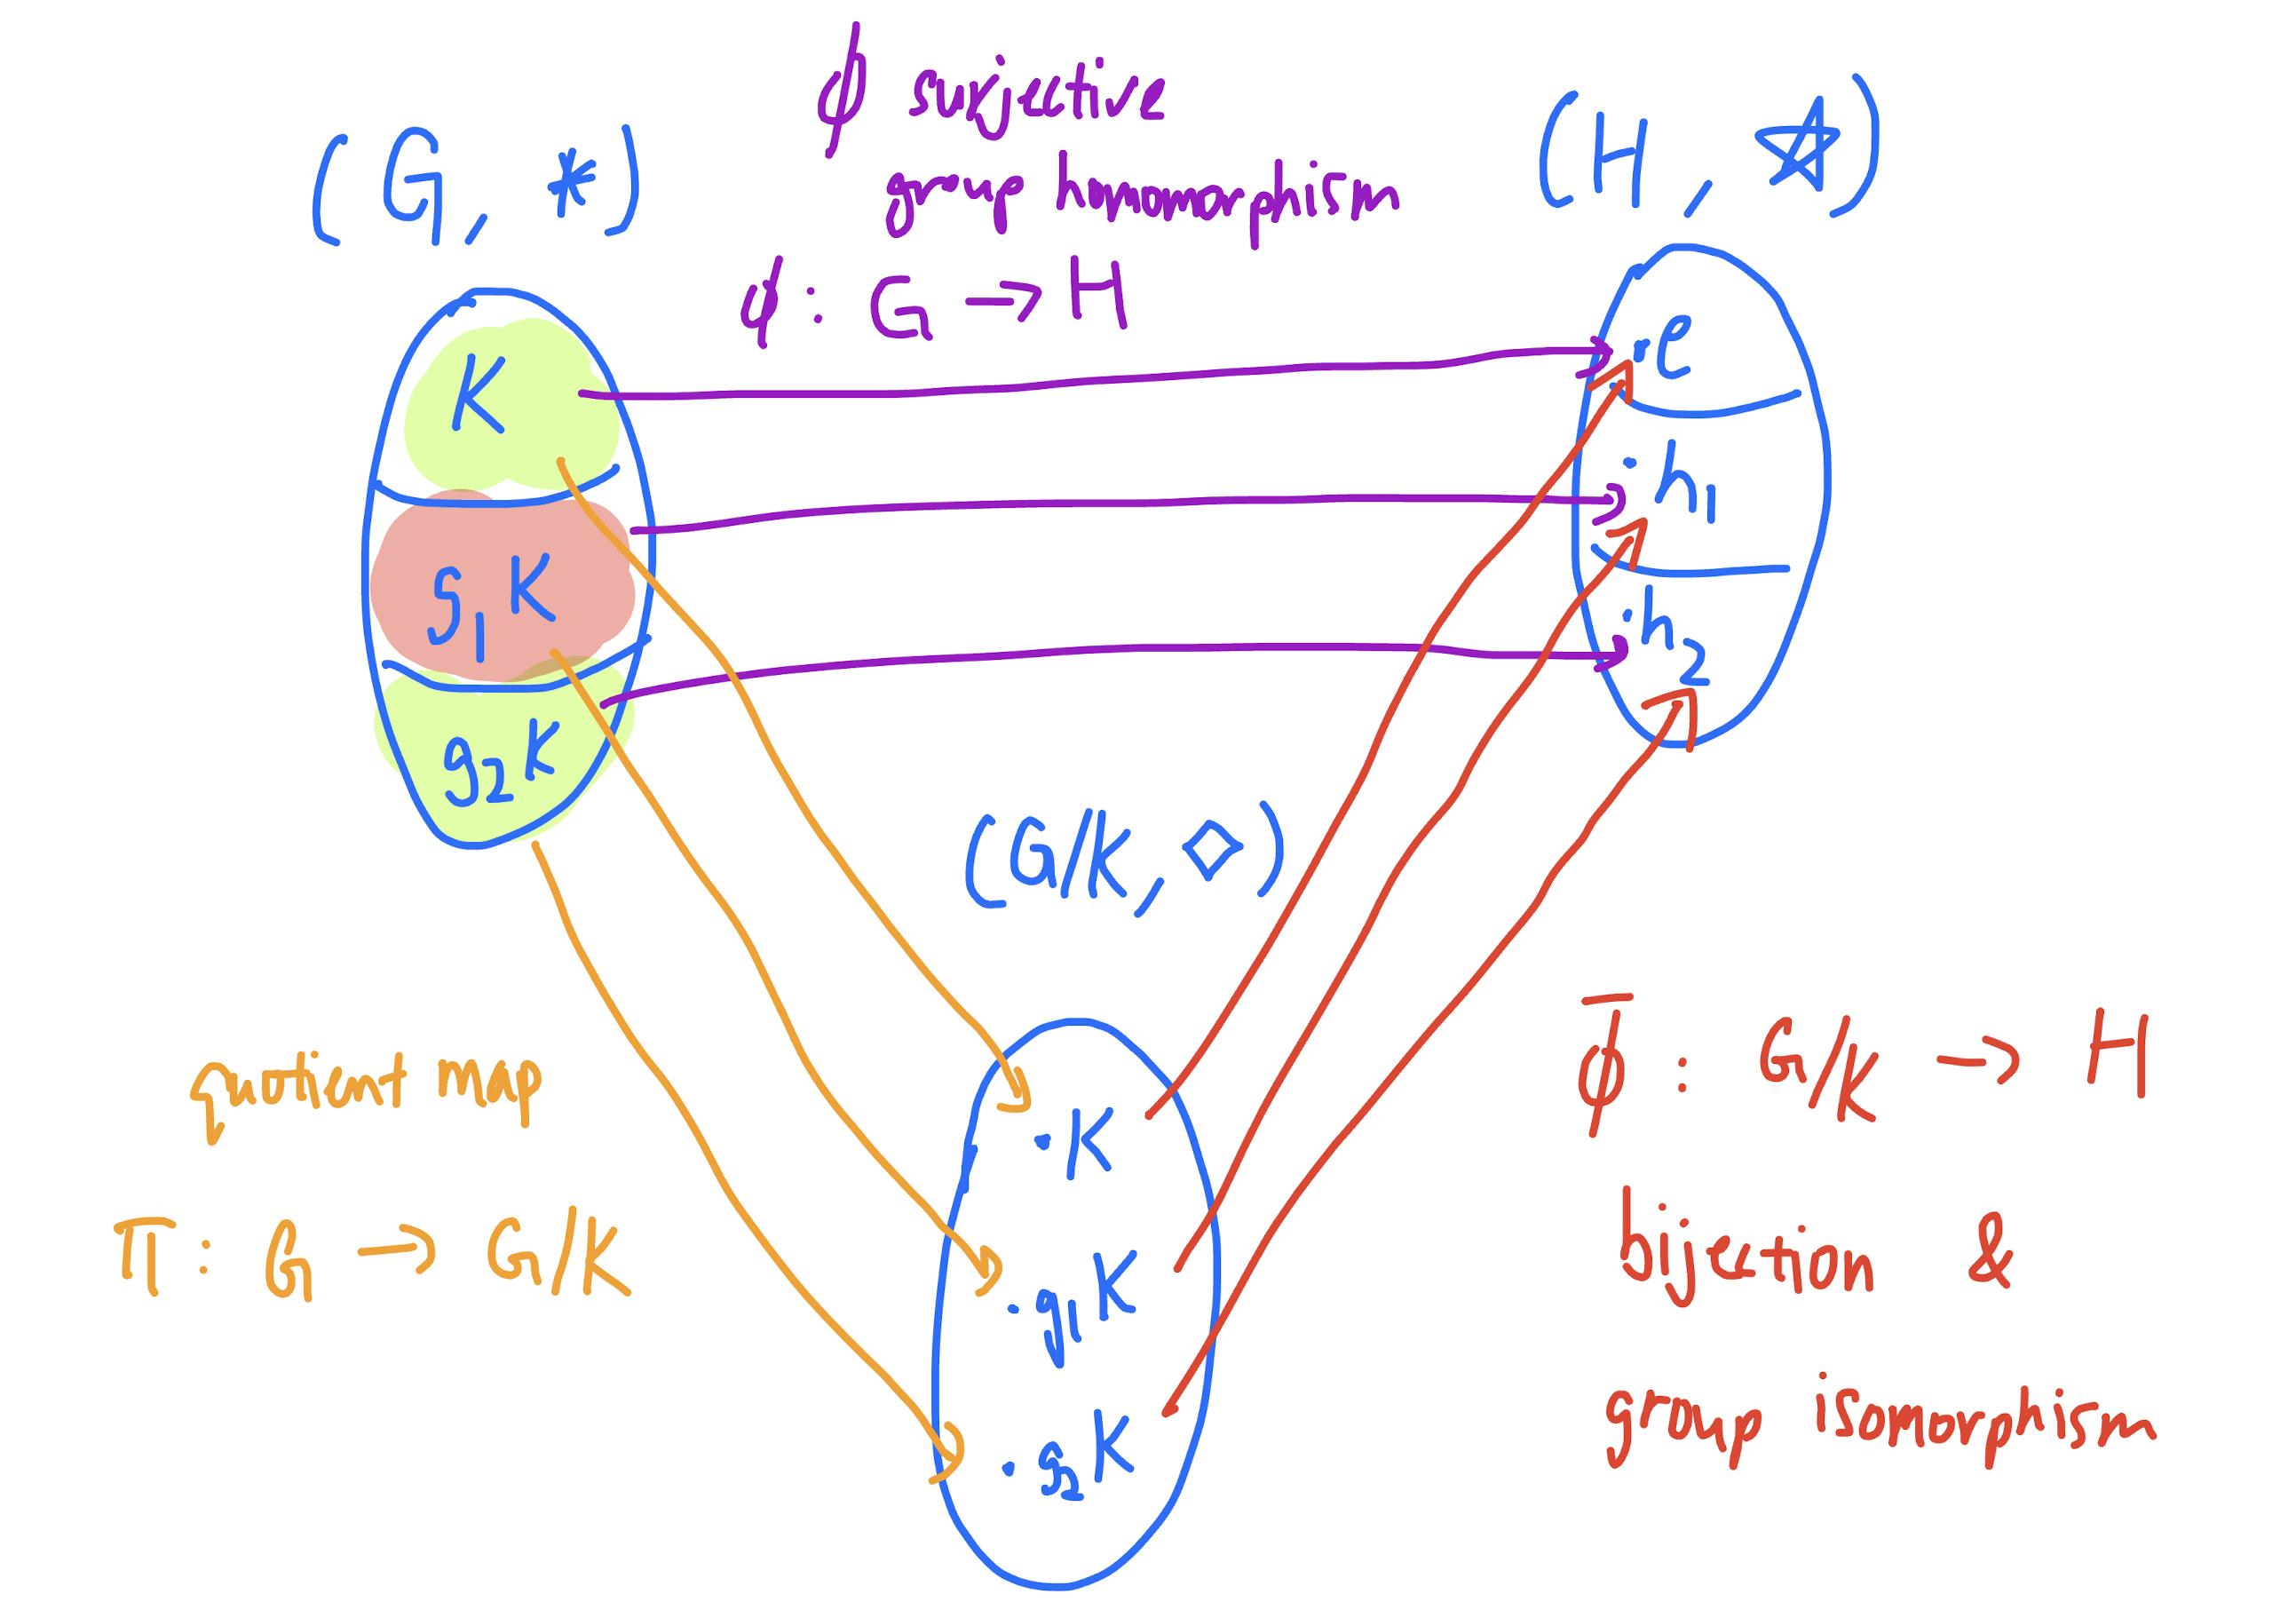
\includegraphics[width=0.8\columnwidth]{5.1}
    \end{center}
    \begin{itemize}[leftmargin=*]
      \item If $\phi$ is not surjective, then replace $H$ with the image $H' = \phi(G)$ in the definition of $\bar{\phi}$.
    \end{itemize}
    \paragraph{Corollary}
      Let $\phi: G \rightarrow H$ and $\psi: G \rightarrow H'$ be two group homomorphisms.
      \begin{itemize}[leftmargin=*]
        \item Suppose $\phi$ and $\psi$ have the same kernel $K$. Then, the images $\phi(G)$ and $\psi(G)$ are isomorphism groups.
        \item If $G$ is a finite group, then
          \[ \abs{\phi(G)} = \abs{\psi(G)} = \abs{G/K} = \abs{G} / \abs{K} \]
      \end{itemize}
\subsection*{The Second Isomorphism Theorem} \noindent
  In this section, $G$ is a group, $M$ is a subgroup of $G$, and $K$ is a normal subgroup of $G$.
  \paragraph{Prop. 59} $MK = KM$ and it is a subgroup of $G$.
  \paragraph{Proposition 60}
    \begin{enumerate}[label=\roman*., leftmargin=*]
      \item The function $\phi: M \rightarrow MK/K$ defined by $\phi(m) = mK$ is a surjective group homomorphism.
      \item The kernel of $\phi$ is $M \cap K$. In particular, it is a normal subgroup of $M$.
    \end{enumerate}
  \subsubsection*{Second Isomorphism Theorem} \noindent
    \[ M / (M \cap K) \simeq (MK)/K \]
\subsection*{The Third Isomorphism Theorem} \noindent
  Let $G$ be a group. Let $M$ and $K$ be normal subgroups of $G$ such that $M \supseteq K$. Then $M/K$ is a normal subgroup of $G/K$ and
  \[ (G/K) / (M/K) \simeq G/M \]
  If $M \not\supseteq K$, then replace $K$ by $M \cap K$, which is a normal subgroup of $G$ contained in $M$.
  \paragraph{Corollary} Let $M$ and $K$ be normal subgroups of $G$ such that $M \supseteq K$. Then there is a surjective group homomorphism
    \[ \phi: G/K \rightarrow G/M \]
    given by $\phi(gK) = gM$.
\subsection*{Euler's totient function} \noindent
  Let $n$ be a positive integer. If $n = 1$, set $\Phi(1) = \{1\}$. Else set
  \[ \Phi(n) = \{x \in \Z: 0 \le x \le n, \gcd(x, n) = 1 \} \]
  \begin{itemize}[leftmargin=*]
    \item Let $*$ denote multiplication modulo $n$. Then $(\Phi(n), \ast)$ is a group.
    \item Let $\phi(n)$ denote the number of elements in $\Phi(n)$.
    \item For prime number $p$, $\Phi(p) = \{1, 2, \cdots p-1\}$, so $\phi(p) = p-1$.
    \item For prime number $p$, let $n=p^r$.
      \[ \phi(p^r) = n - \frac{n}{p} = p^r \left( 1 - \frac{1}{p} \right) = p^{r-1}(p-1) \]
  \end{itemize}
  \subsubsection*{Euler's theorem} \noindent
    Let $x$ be an integer such that $\gcd(x,n) = 1$. Then
    \[ x^{\phi(n)} \equiv 1 \pmod{n} \]
  \subsubsection*{Calculating $\phi(n)$} \noindent
    Suppose $n = p_1^{r_1} p_2^{r_2} \cdots p_n^{r_n}$. Then
    \begin{align*}
      \phi(n) &= n \left(1 - \frac{1}{p_1}\right) \left(1 - \frac{1}{p_2}\right) \cdots \left(1 - \frac{1}{p_k}\right) \\
              &= \phi(p_1^{r_1}) \phi(p_2^{r_2}) \cdots \phi(p_k^{r_k})
    \end{align*}
    \paragraph{Example} Compute $43^{866} \pmod{360}$.
      \begin{itemize}[leftmargin=*]
        \item $360 = 2^3 \cdot 3^2 \cdot 5$ so
          \[ \phi(360) = 360 \left(1 - \frac{1}{2}\right) \left(1 - \frac{1}{3}\right) \left(1 - \frac{1}{5}\right) = 96 \]
        \item Since $\gcd(43, 360) = 1$, Euler's theorem gives $43^{96} \equiv 1 \pmod{360}$.
        \item We have $866 = 96(9) + 2$ so
          \begin{align*}
            43^{866} &\equiv 43^{96(9) + 2} \equiv (43^{96})^9 43^2 \\
                     &\equiv 1^9 43^2 \equiv 49 \pmod{360}
          \end{align*}
      \end{itemize}
\subsection*{Automorphism groups} \noindent
  Let $(G,\ast)$ be a group. An isomorphism $\phi: G \rightarrow G$ is called an automorphism of $G$. We denote the set of automorphisms of $G$ by
  \[ \Aut{G} = \{ \phi: G \rightarrow G: \phi \text{ is an isomorphism} \} \]
  \subsubsection*{Isomorphism facts}
    \begin{itemize}[leftmargin=*]
      \item Identity map $\mathrm{id}_G$ is an isomorphism.
      \item Composition of isomorphisms is an isomorphism, i.e. $\circ$ is a binary operation on $\Aut{G}$.
      \item Inverse of an isomorphism is an isomorphism.
    \end{itemize}
    \paragraph{Proposition} $(\Aut{G}, \circ)$ forms a group.
      \begin{itemize}[leftmargin=*]
        \item It is called the automorphism group of $G$.
        \item A subgroup $A$ of $(\Aut{G}, \circ)$ is called an automorphism subgroup.
      \end{itemize}
  \subsubsection*{Inner automorphism} \noindent
    Let $G$ be a group and let $g \in G$. Then $\phi_g: G \rightarrow G$ given by
    \[ \phi_g(x) = gxg^{-1} \]
    is a group automorphism. It is called an inner automorphism of $G$.
    \begin{itemize}[leftmargin=*]
      \item Let $\Inn{G} = \{ \phi_g: g \in G \}$ be the set of inner automorphisms.
      \item The subset $\Inn{G}$ is a normal subgroup of $(\Aut{G}, \circ)$.
    \end{itemize}
    \paragraph{Proposition} The map $T: G \rightarrow \Inn{G}$ given by $T(g) = \phi_g$ is a surjective group homomorphism whose kernel is the center of the group
      \[ Z(G) = \{z \in G: gz = zg \text{ for all } g \in G\} \]
      By the first isomorphism theorem,
      \[ G/Z(G) \simeq \Inn{G} \]
\subsection*{The Sylow Theorems}
  \paragraph{Notation} Let $n$ be a positive integer. Suppose $p^e$ divides $n$, but $p^{e+1}$ does not divide $n$. We write $p^e \vv n$. Alternatively, n = $p^e m$ where $p \not\vert\; m$.
  \subsubsection*{Definition} \noindent
    Let $G$ be a finite group of order $n$. Let $p$ be a prime divisor of $n$. Let $H$ be a subgroup of order of $p^e$.
    \begin{itemize}[leftmargin=*]
      \item $H$ is called a $p$-subgroup of $G$.
      \item If $p^e \vv n$, then $H$ is called a Sylow $p$-subgroup of $G$.
    \end{itemize}
    \paragraph{Example} Let $G = S_9$. It has order $9! = 2^7 3^4 5^1 7^1$.
      \begin{itemize}[leftmargin=*]
        \item A subgroup of order $2^5$ is a 2-subgroup.
        \item A subgroup of order $2^7$ is a Sylow 2-subgroup.
      \end{itemize}
  \subsubsection*{First Sylow Theorem} \noindent
    Let $G$ be a group of order $n$. Let $p$ be a prime divisor of $n$. Then $G$ contains a Sylow $p$-subgroup.
    \paragraph{Corollary} Let $G$ be a finite group of order $n$. Let $p$ be a prime divisor of $n$. If $p^d \vert n$, then $G$ contains a subgroup of order $p^d$.
  \subsubsection*{Definition} \noindent
    Let $P$ be a subgroup of $G$. Let $g \in G$. Then $gPg^{-1}$ is a subgroup of $G$ called a conjugate of $P$. Let $P$ be a Sylow $p$-subgroup. Then a conjugate $gPg^{-1}$ is also a Sylow $p$-subgroup.
  \subsubsection*{Theorem 94} \noindent
    Let $G$ be a group of order $n$. Let $\{P_1, P_2, \cdots, P_r\}$ be all the distinct conjugates of a Sylow $p$-subgroup $P = P_1$.
    \begin{enumerate}[label=\roman*., leftmargin=*]
      \item Let $Q$ be a $p$-subgroup of $G$. Then $Q \subseteq P_i$ for some $i$.
      \item (Second) If $Q$ is a Sylow $p$-subgroup of $G$, then $Q = P_i$ for some $i$.
      \item (Third) Let $r$ denote the number of Sylow $p$-subgroups of $G$. Then
        \[ r \equiv 1 \pmod{p} \text{ and } r \vert [G:P] \]
    \end{enumerate}
    \paragraph{Corollary 95} Let $P$ be a Sylow $p$-subgroup of a finite group $G$. Then $P$ is a normal subgroup $\iff P$ is the unique Sylow $p$-subgroup of $G$.
\end{multicols*}
\end{document}
